\documentclass[sans,14pt]{beamer}
\usepackage{pgfpages}
%\setbeameroption{show notes on second screen}
%\setbeameroption{show notes}
\setbeameroption{hide notes}

\usepackage{etex}


\usepackage{fixltx2e} % for \textsubscript


%% Format the bibliography
\usepackage[backend=bibtex,style=alphabetic]{biblatex}
\addbibresource{references}
\setbeamercolor*{bibliography entry title}{fg=MyDarkGrey}
\setbeamercolor*{bibliography entry author}{fg=black}
\setbeamercolor*{bibliography entry location}{fg=black}
\setbeamercolor*{bibliography entry note}{fg=black}
\setbeamertemplate{bibliography item}[text]

% Space between label and reference
\setlength{\biblabelsep}{-15pt}


\mode<presentation>
{
  \usetheme{Copenhagen}
  \usecolortheme{beaver}
  \usefonttheme[onlymath]{serif}
}

%% Change bullet points style
%\setbeamertemplate{itemize items}[triangle]
\setbeamertemplate{itemize items}{{\textemdash}}
\setbeamercolor*{item}{fg=MyDarkGrey}

%% Remove navigation symbols
\setbeamertemplate{navigation symbols}{}
\setbeamertemplate{headline}{}

%% Use only frame number (no total frame count) in footer
\setbeamertemplate{footline}{%
  \raisebox{5pt}{\makebox[\paperwidth]{\hfill\makebox[20pt]{
        \scriptsize\insertframenumber}}}
}

% Adjust margin of itemize environment
\setlength{\leftmargini}{0pt}
\setlength{\leftmarginii}{10pt}
\setlength{\leftmarginiii}{17pt}

%% Adjust font sizes
\setbeamerfont{frametitle}{size=\Large}
\setbeamerfont{normal text}{size=\small}
\setbeamerfont{itemize/enumerate body}{size=\small}
\setbeamerfont{itemize/enumerate subbody}{size=\small}
\setbeamerfont{itemize/enumerate subsubbody}{size=\footnotesize}

%%% To use the Cabin-Condensed fonts
%%% More fonts: see http://www.tug.dk/FontCatalogu
% \usepackage[latin1]{inputenc}
% \usepackage[T1]{fontenc}
% \usepackage[sfdefault]{cabin} 
\usepackage{PTSans} 
\usepackage{PTSansNarrow} 
\renewcommand*\familydefault{\sfdefault} %% Only if the base font of the document is to be sans serif
\usepackage[T1]{fontenc}

\newenvironment{ptnormal}{\fontfamily{PTSans-TLF}\selectfont}{\par}


\usepackage{amsmath}
\usepackage{amsfonts}
\usepackage{amssymb}
\usepackage{amsthm}
\usepackage{bm}
\usepackage{booktabs}
\usepackage{color}
\usepackage{epstopdf}
\usepackage{fancyhdr}
\usepackage{fancybox}
\usepackage[all]{xy}
\usepackage{graphicx}
\usepackage{multirow}
\usepackage[normalem]{ulem}
\usepackage{url}
\usepackage{dsfont}
%


% tikzmark command, for shading over items
\usepackage{tikz}
\usetikzlibrary{calc}
\newcommand{\tikzmark}[1]{\tikz[overlay,remember picture] \node (#1) {};}
\usetikzlibrary{decorations.pathreplacing} % for curly braces
\usepackage[framemethod=tikz]{mdframed} % for fancy title page and other boxes

%% Subfigures
\usepackage[labelformat=simple,caption=false,textfont=scriptsize]{subfig}
\renewcommand{\thesubfigure}{\relax} % do not number captions of
                                     % subfloats


%% to write text at the bottom of a beamer slide
%\def\writeatbottom#1{\vskip 0pt plus 1filll \scriptsize #1}

\newcommand{\topspace}{\rule{0pt}{2.6ex}}
\newcommand{\botspace}{\rule[-1.2ex]{0pt}{0pt}}


%%% Colors
%\usepackage{color}
\definecolor{MyBlue}{rgb}{0.27,0.62,0.73}%{0.,0.2,0.4} 
\definecolor{Aubergine}{rgb}{0.47,0.13,0.44} % 119 33 111
\definecolor{MyTurq}{rgb}{0.,0.8,0.8} 
\definecolor{MyDarkGrey}{rgb}{0.3,0.3,0.3} 
\definecolor{MyMedGrey}{rgb}{0.6,0.6,0.6} 
\definecolor{MyLightGrey}{rgb}{0.95,0.95,0.95} 
\definecolor{MyDarkRed}{rgb}{0.8,0.,0.} 
\definecolor{MyOrange}{rgb}{0.93,0.56,0.25}
\definecolor{MyPink}{rgb}{0.73,0.27,0.39}
\definecolor{MyLightYellow}{HTML}{FFFFCC}
%\usepackage[colorlinks=true,citecolor=MyTurq]{hyperref}
\AtEveryCite{\color{MyMedGrey}}

\newcommand{\blue}[1]{{\color{MyBlue}{\textbf{#1}}}}
\newcommand{\red}[1]{{\color{MyOrange}{\textbf{#1}}}}
\newcommand{\black}[1]{{\color{MyDarkGrey}{\textbf{#1}}}}
\newcommand{\yellow}[1]{{\color{MyLightYellow}{\textbf{#1}}}}

\newcommand{\TODO}{{\color{MyDarkRed}{TODO~}}}

\setbeamercolor{normal text}{fg=MyDarkGrey}
\setbeamercolor{frametitle}{fg=Aubergine}

%%% ---- Titre des slides  (underline) ----------------
\setbeamertemplate{frametitle}{%
    \usebeamerfont{frametitle}\insertframetitle\strut%
    \vskip-.05\baselineskip%
    \leaders\vrule width \paperwidth\vskip1.pt%
    \vskip0pt%
    \nointerlineskip
}
%%% ---------------------------------------------------


% --- Math symbols -------------------------------------------------------------
\newcommand{\EE}{{\mathbb E}}
\newcommand{\PP}{{\mathbb P}}
\newcommand{\NN}{{\mathbb N}}
\newcommand{\RR}{{\mathbb R}}

\newcommand{\avec}{\vec{a}}
\newcommand{\alphavec}{\vec{\alpha}}
\newcommand{\betavec}{\vec{\beta}}
\newcommand{\cvec}{\vec{c}}
\newcommand{\fvec}{\vec{f}}
\newcommand{\muvec}{\vec{\mu}}
\newcommand{\mvec}{\vec{m}}
\newcommand{\rvec}{\vec{r}}
\newcommand{\thetavec}{\vec{\theta}}
\newcommand{\xvec}{\vec{x}}
\newcommand{\yvec}{\vec{y}}
\newcommand{\wvec}{\vec{w}}
\newcommand{\uvec}{\vec{u}}
\newcommand{\vvec}{\vec{v}}
\newcommand{\zvec}{\vec{z}}

% \newcommand{\amat}{{\mathbf A}}}
% \newcommand{\dmat}{{\mathbf D}}
% \newcommand{\gmat}{{\mathbf G}}
% \newcommand{\kmat}{{\mathbf K}}
% \newcommand{\lmat}{{\mathbf L}}
% \newcommand{\mmat}{{\mathbf M}}
% \newcommand{\wmat}{{\mathbf W}}
% \newcommand{\xmat}{{\mathbf X}}

\newcommand{\aset}{\mathcal{A}}
\newcommand{\cset}{\mathcal{C}}
\newcommand{\dset}{\mathcal{D}}
\newcommand{\fcal}{\mathcal{F}}
\newcommand{\hcal}{\mathcal{H}}
\newcommand{\ncal}{\mathcal{N}}
\newcommand{\nset}{\mathcal{N}}
\newcommand{\rcal}{\mathcal{R}}
\newcommand{\sset}{\mathcal{S}}
\newcommand{\vset}{\mathcal{V}}
\newcommand{\tset}{\mathcal{T}}
\newcommand{\xcal}{\mathcal{X}}
\newcommand{\ycal}{\mathcal{Y}}

\newcommand{\lzeronorm}[1]{\left|\left|#1\right|\right|_0}
\newcommand{\lonenorm}[1]{\left|\left|#1\right|\right|_1}
\newcommand{\ltwonorm}[1]{\left|\left|#1\right|\right|_2}

\usepackage{bbm}
\newcommand{\indic}{\mathbbm{1}}

\DeclareMathOperator*{\argmin}{arg\,min}
\DeclareMathOperator*{\argmax}{arg\,max}
\graphicspath{{./figures/}}

% ------------------------------------------------------------------------------



% \newcommand{\source}[1]{\begin{textblock*}{4cm}(8.7cm,8.6cm)
%     \begin{beamercolorbox}[ht=0.5cm,right]{framesource}
%       \usebeamerfont{framesource}\usebeamercolor[fg]{framesource} Credits: {#1}
%     \end{beamercolorbox}
% \end{textblock*}}




\newcommand{\mytitle}{Fondamentaux du Machine Learning}
\author[Walter]{Thomas Walter \and  Chlo\'e-Agathe~Azencott \and Florian Massip} 
\institute[CBIO]{\inst{1} Centre for Computational Biology(CBIO), Mines Paris, PSL University\and %
                      \inst{2} Institut Curie\and
                      \inst{3} U900 - INSERM}

\date{\small November 2022}

\begin{document}
{

  \begin{frame}[plain]
    \fontfamily{PTSansNarrow-TLF}\selectfont
    \begin{center}
      {\ptnormal{\textit{Formation Chef de Projet IA}}}
    \end{center}

    \vspace{70pt}

    \centerline{{\Large \bf \mytitle}}

    \vspace{15pt}

    \centerline{\insertauthor}

    \vspace{15pt}

    {\footnotesize
      \centerline{Center for Computational Biology (CBIO)}
    
      \centerline{Mines Paris -- Institut Curie -- INSERM U900}

      \centerline{PSL Research University \& PR[AI]RIE, Paris, France}
    }

    \centerline {\insertdate}

\end{frame}

% Do not count title slide when numbering frames
\addtocounter{framenumber}{-1}


% Overview
\begin{frame}
  \frametitle{Programme}

  \begin{itemize}
  \item Introduction à l'apprentissage automatique
  \item \blue{Cours 1 :} Minimisation du risque empirique 
  \item \blue{Cours 2 :} Régularisation et sélection de modèle
  \item \blue{Cours 3 :} Arbres et méthodes ensemblistes
  \item \blue{Cours 4 :} Méthodes à noyaux 
  \item \blue{Cours 5 :} Réduction de dimension
  \item \blue{Cours 6 :} Clustering
  \item Travaux pratiques : mise en œuvre des notions et algorithmes avec scikit-learn (Python numérique).
\end{itemize}
\end{frame}






\begin{frame}
  \begin{center}
    \large{Arbres de décision}
  \end{center}
\end{frame}

\begin{frame}
  \frametitle{Exemple}
  \begin{center}
    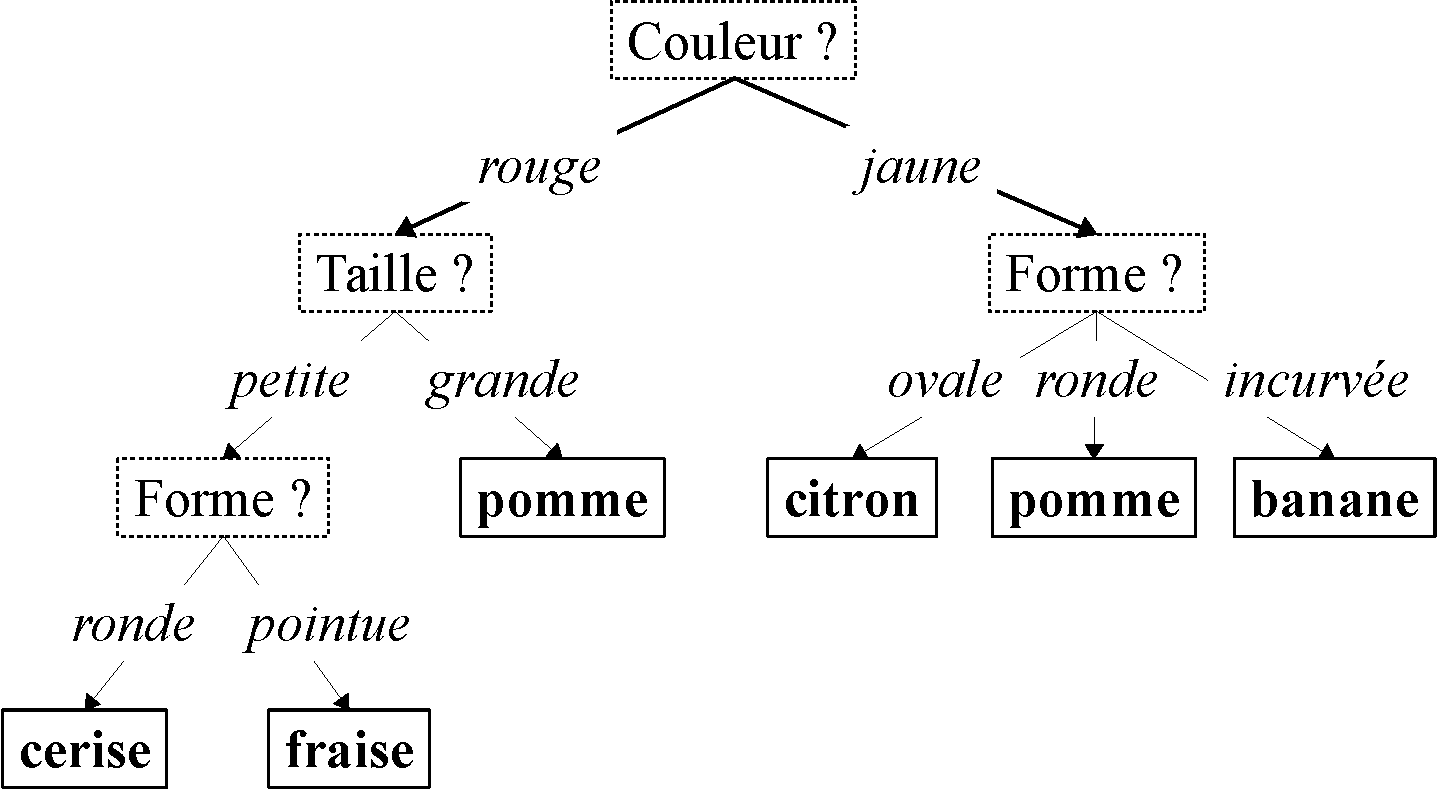
\includegraphics[width=.7\textwidth]{figures/fruit_tree}
  \end{center}
\end{frame}

  \begin{frame}
    \frametitle{Les arbres de décision}
  \begin{itemize}
    \item Méthode hiérarchique
    \item Série successive de tests conditionnels.
    \item Souvent utilisé en dehors de la classification automatique : 
    \begin{itemize}
      \item aide à la décision
      \item formalisation d'un raisonnement
    \end{itemize}
  \end{itemize}
\end{frame}


\begin{frame}
  \frametitle{Les arbres de décision pour la classification}
  \begin{center}
    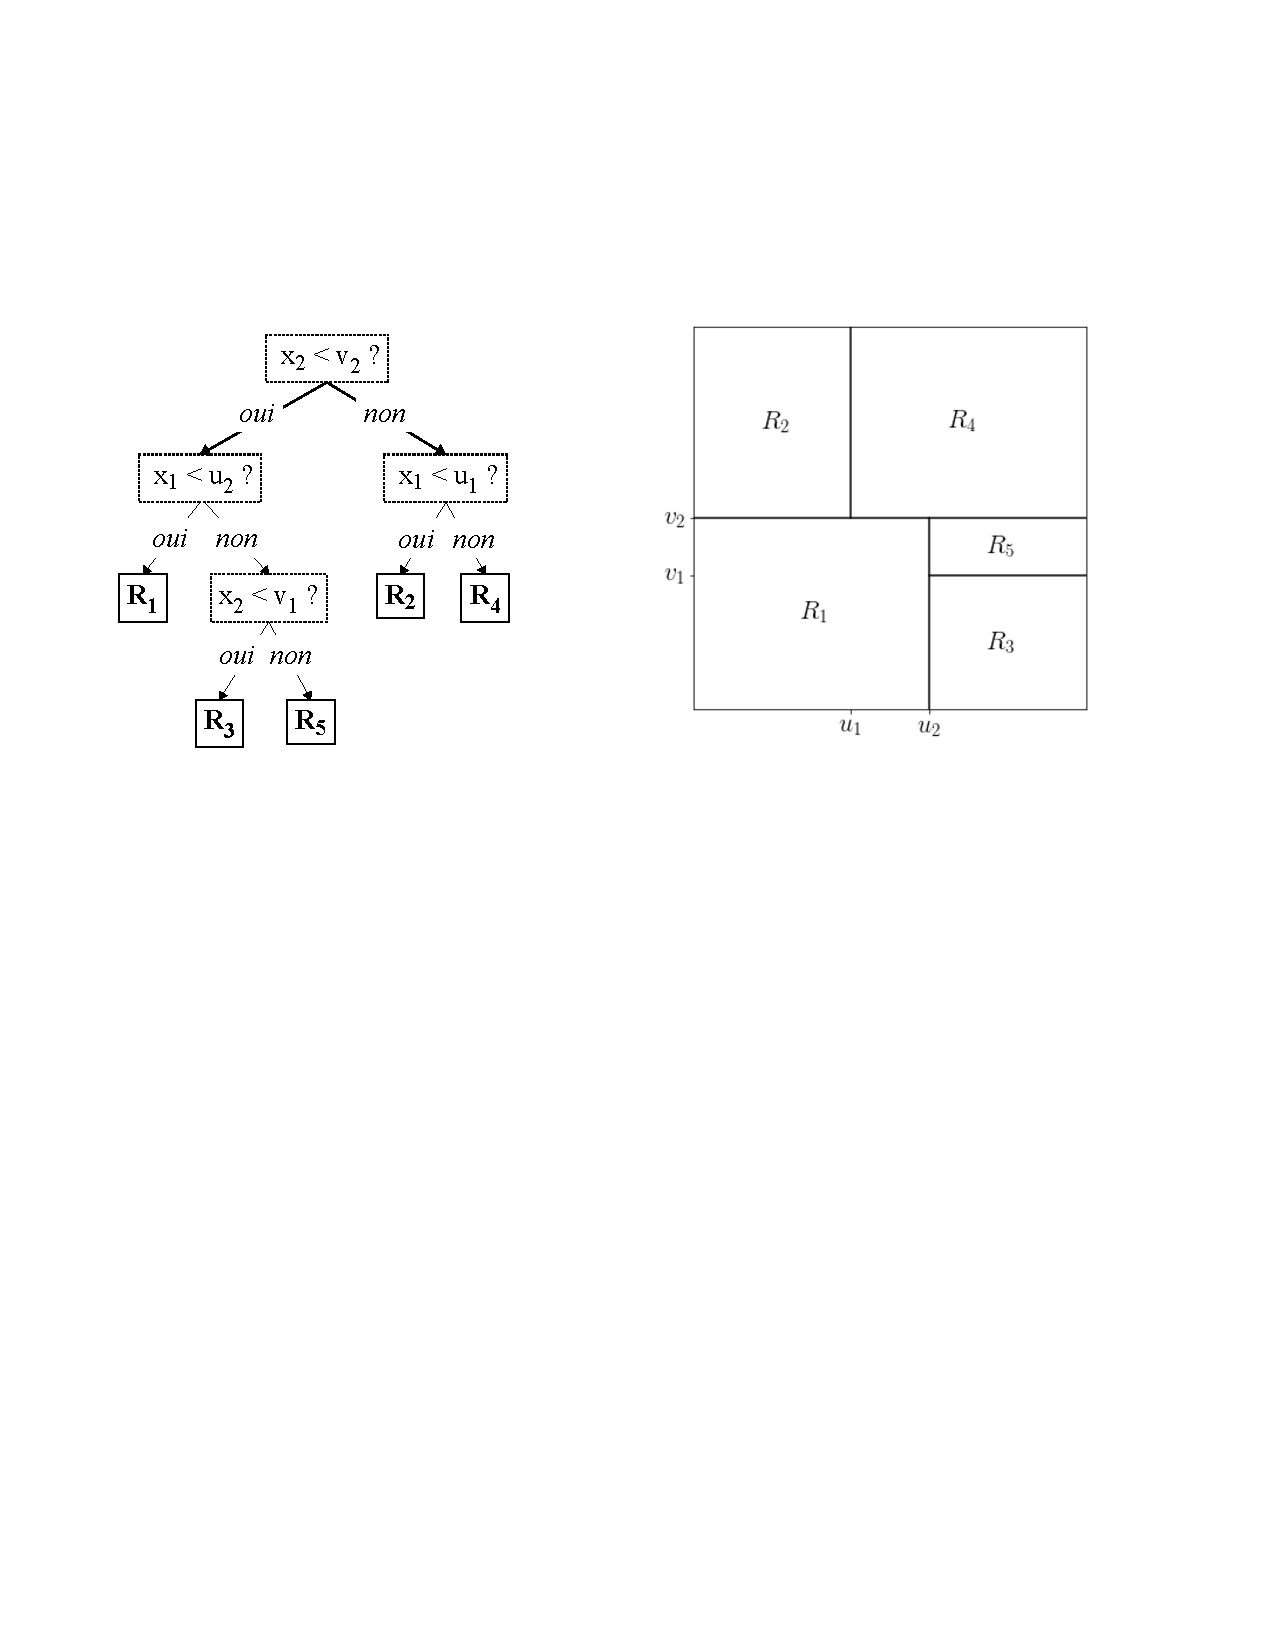
\includegraphics[width=.7\textwidth]{figures/arbre}
  \end{center}
  \begin{itemize}
    \item En classification, les tests correspondent à des seuils, appliqués aux descripteurs. 
    \item Chaque arbre de décision correspond à une partition de l'espace des descripteurs.
    \item On peut assigner une classe à chaque feuille. 
  \end{itemize}
\end{frame}


\begin{frame}
  \frametitle{Les arbres de décision - avantages}
  \begin{itemize}
    \item Classification en classes multiples
    \item Interprétabilité
    \item Traitement de variables catégoriques
    \item Mélange de types de variables
  \end{itemize}
\end{frame}

\begin{frame}
  \frametitle{Construction des arbres}
  \begin{itemize}
    \item CART: Classification and regression trees
    \item A chaque étape, une région est divisée en deux. 
    \item Pour ce, il faut choisir un descripteur $x_j$ et un seuil $s$. 
    \item Ce choix est fait pour optimiser un critère, calculé sur les régions qui résultent de ce seuillage. 
  \end{itemize}
\end{frame}

\begin{frame}
  \frametitle{Split : critère de régression}
  \begin{itemize}
    \item Un suppose qu'un split $(j,s)$ génère deux régions $R_1$ et $R_2$. 
    \item Dans le cas d'une regression, on calcule alors les moyennes $\overline{y_1}$ et $\overline{y_2}$ des étiquettes dans les régions $R_1(j,s)$ et $R_2(j,s)$. 
    \item Le critère à minimiser par $(j,s)$:
    \begin{equation*}
    (j,s)^{\ast} = \argmin_{j,s}\sum_{\xvec_k \in R_1} (y_k-\overline{y_1})^2 + \sum_{\xvec_k \in R_2}(y_k-\overline{y_2})^2
    \end{equation*}
    où $\overline{y_1}, \overline{y_2}, R_1, R_2$ dépendent de $(j,s)$. 
  \end{itemize}
\end{frame}

\begin{frame}
  \frametitle{Split : critère de classification}
  \begin{itemize}
    \item \blue{Erreur de classification} :  
    \begin{equation*}
    Imp(R) = 1- \max_{c=1, \ldots C}p_c(R)
    \end{equation*}
    avec $p_c(R)$ la probabilité (proportion) de la classe $c$ dans $R$. 
    \item Ce critère est:
    \begin{itemize}
      \item 0 si toutes les instances appartiennent à la même classe.
      \item $1-\frac{1}{C}$ si les classes sont distributées équitablement.
    \end{itemize}
  \end{itemize}
\end{frame}

\begin{frame}
  \frametitle{Split : critère de classification}
  \begin{itemize}
    \item \blue{Entropie} :  
    \begin{equation*}
      Imp(R) = -\sum_{c=1}^{C}p_c(R)\log_2p_c(R)
    \end{equation*}
    \item Ce critère est:
    \begin{itemize}
      \item 0 si toutes les instances appartiennent à la même classe.
      \item $\log_2{C}$ si les classes sont distributées équitablement.
    \end{itemize}
  \end{itemize}
\end{frame}


\begin{frame}
  \frametitle{Split : critère de classification}
  \begin{itemize}
    \item \blue{Critère de impureté GINI}: 
    \begin{equation*}
    Imp(R) = \sum_{c=1}^{C}p_c(R)(1-p_c(R))
    \end{equation*}
    avec $p_c(R)$ la probabilité (proportion) de la classe $c$ dans $R$.     
    \item Ce critère est:
    \begin{itemize}
      \item 0 si toutes les instances appartiennent à la même classe.
      \item $1-\frac{1}{C}$ si les classes sont distributées équitablement.
    \end{itemize}
  \end{itemize}
\end{frame}

\begin{frame}
  \frametitle{Split : critère de classification}
  \begin{itemize}
    \item Le critère à minimiser par $(j,s)$:
    \begin{equation*}
    (j,s)^{\ast} = \argmin_{j,s}\frac{|R_1|}{n}Imp(R_1) + \frac{|R_2|}{n}Imp(R_2)
    \end{equation*}
    avec $|\cdot|$ le cardinal et $R_1, R_2$ des fonctions de $(j,s)$. 
    \item On itère sur toutes les valeurs possibles de j et toutes les valeurs possibles de $s$ pour déterminer le couple (j, s) qui minimise le critère.
  \end{itemize}
\end{frame}

\begin{frame}
  \frametitle{Critère d'impureté GINI: Exemple}  
   \begin{figure} 
     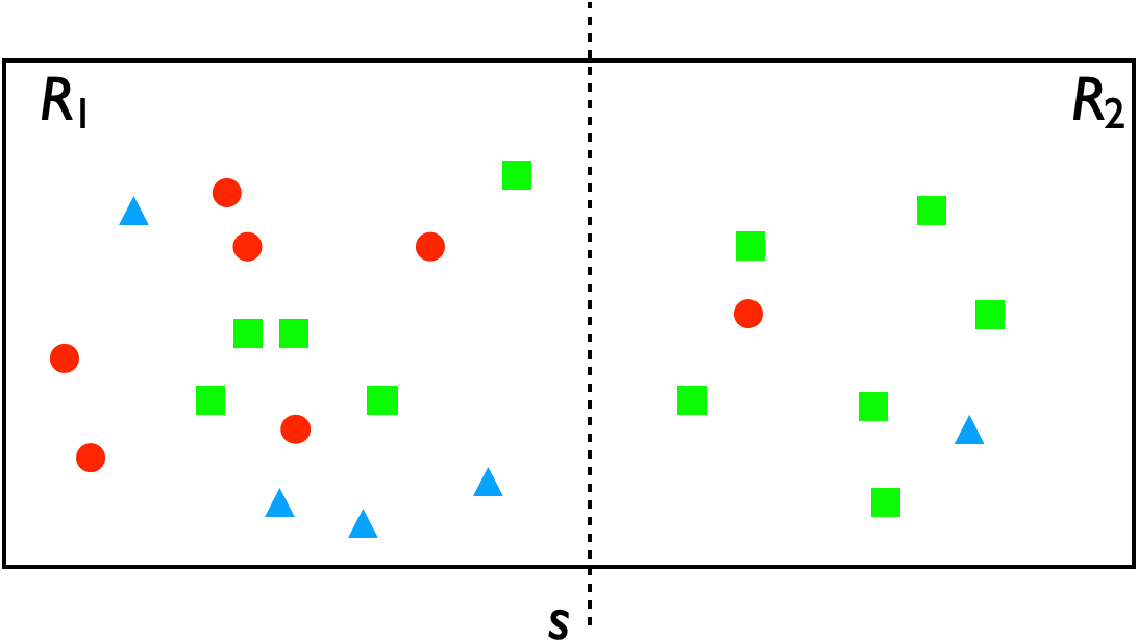
\includegraphics[width=0.8\textwidth]{GINI_example.pdf}
     \caption{Exemple pour le calcul de l'impureté GINI}
   \end{figure}
   % \begin{eqnarray}
   % GI(R_1) &=& \frac{2}{5}\frac{3}{5} + \frac{4}{15}\frac{11}{15} + \frac{1}{3}\frac{2}{3} = 0.658\nonumber \\
   % GI(R_2) &=& \frac{1}{8}\frac{7}{8} + \frac{1}{8}\frac{7}{8} + \frac{6}{8}\frac{2}{8} = 0.40625\nonumber \\
   % GI(j,s) &=& \frac{15}{23}GI(R_1) + \frac{8}{23}GI(R_2) = 0.57
   % \end{eqnarray}
\end{frame}

\begin{frame}
  \frametitle{Critère d'impureté GINI: Exemple} 
   \begin{figure}
     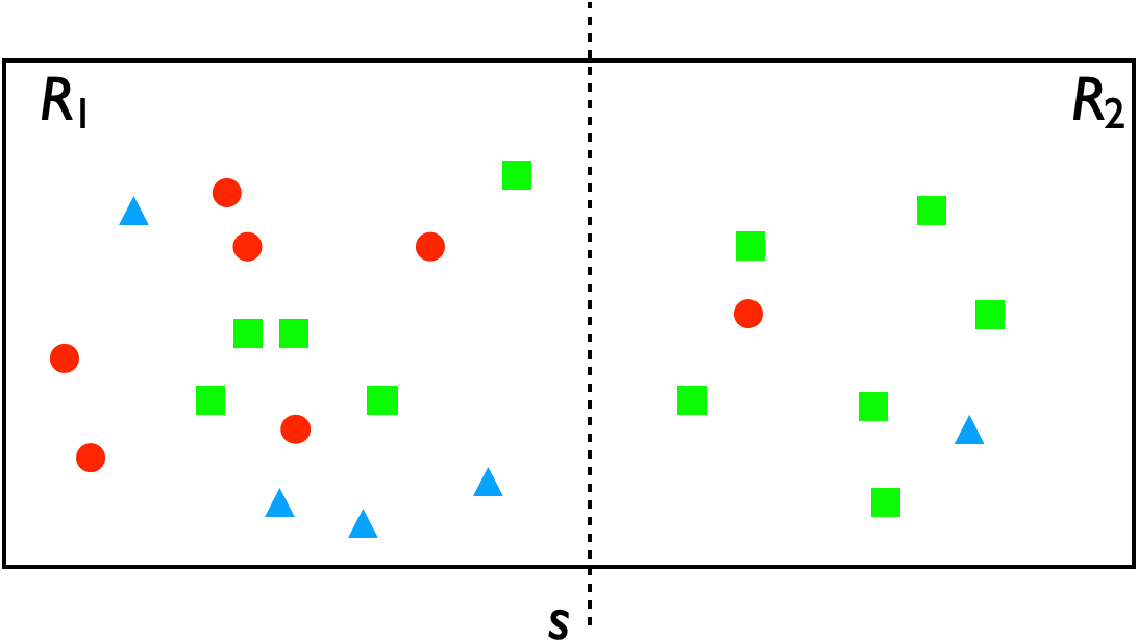
\includegraphics[width=0.4\textwidth]{GINI_example.pdf}
     \caption{Exemple pour le calcul de l'impureté GINI}
   \end{figure}
   \begin{eqnarray}
   GI(R_1) &=& \frac{2}{5}\cdot\frac{3}{5} + \frac{4}{15}\cdot\frac{11}{15} + \frac{1}{3}\cdot\frac{2}{3} = 0.658\nonumber \\
   GI(R_2) &=& \frac{1}{8}\cdot\frac{7}{8} + \frac{1}{8}\cdot\frac{7}{8} + \frac{6}{8}\cdot\frac{2}{8} = 0.40625\nonumber \\
   GI(j,s) &=& \frac{15}{23}GI(R_1) + \frac{8}{23}GI(R_2) = 0.57 \nonumber
   \end{eqnarray}
\end{frame}


\begin{frame}
  \frametitle{Critère d'arrêt}
  \begin{itemize}
    \item Une classe par feuille : risque de sur-apprentissage
    \item Profondeur fixe
    \item Nombre d'observation par feuille
  \end{itemize}
\end{frame}


% \begin{frame}[t]
%   \frametitle{Construction d'un arbre}
%   \begin{itemize}
%   \item Exemple :
%     \begin{itemize}
%     \item 4 petites pommes jaunes, 5 grosses pommes vertes, 3 bananes, 6 mini-concombres
%     \item attributs : vert/jaune, rond/pas rond, gros/petit
%     \end{itemize}
%   \end{itemize}
% \end{frame}

\begin{frame}
  \frametitle{Avantages / Inconvénients}
  \begin{itemize}
    \item Avantages : 
    \begin{itemize}
      \item Simplicité
      \item Interpretabilité
      \item Peut gérer des variables catégoriques et coninues.
    \end{itemize}
    \item Inconvénients : 
    \begin{itemize}
      %\item Temps de calcul sous-optimal (en inférence)
      \item Grand risque de sur-apprentissage
      \item Généralement une performance limitée
  \end{itemize}
  \end{itemize}
\end{frame}

\begin{frame}
  \begin{center}
    \large{2. Méthodes ensemblistes}
  \end{center}
\end{frame}

\begin{frame}
  \frametitle{Sagesse des foules}
  \begin{center}
    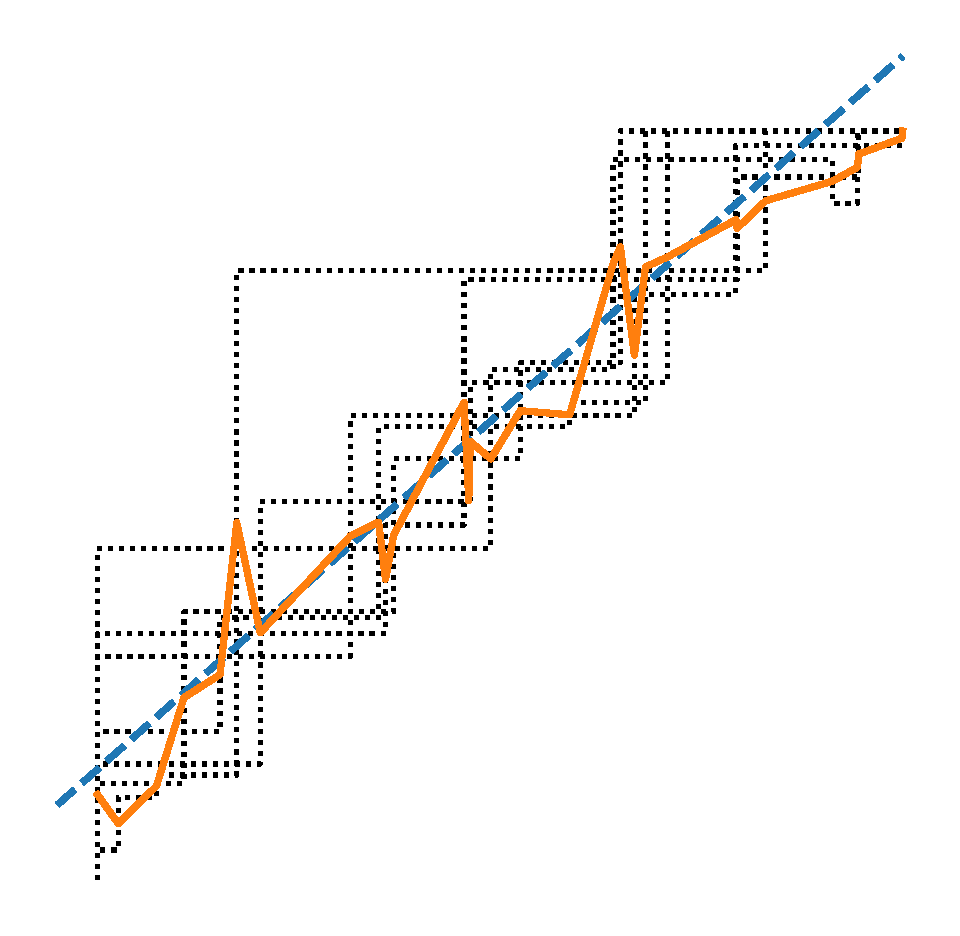
\includegraphics[width=.5\textwidth]{figures/crowd_diagonal}
  \end{center}
  \begin{itemize}
  \item Combiner des \blue{apprenants faibles}.
  \item Exemple: fonction diagonale, approchée par des fonctions en esaclier. 
  \item Principe démocratique. 
  \end{itemize}
\end{frame}

\begin{frame}
  \frametitle{Bagging}
  \begin{itemize}
    \item Bagging = Bootstrap + aggregation
    \item On considère une partie de $\dset$ (e.g. $80\%$) par échantillonage "bootstrap" (avec remise). 
    \item On entraîne un arbre de décision. 
    \item On reitère cette procédure pour obtenir un ensemble d'arbres. 
    \item Le résultat est obtenu par vote majoritaire (classification) ou en moyennant (régression).  
    \item Faire une moyenne de modèles est effectivement une technique de régularisation. 
  \end{itemize}
\end{frame}

\begin{frame}
  \frametitle{Forêts aléatoires}
  \begin{itemize}
    \item En plus du bagging, on peut à chaque noeud tirer aléatoirement des variables parmi lesquels la variable optimale est trouvée. 
    \item Le résultat : \blue{les forêts aléatoires}. 
    \item Les arbres sont plus différents et couvrent "différent aspects" des données. 
    \item En pratique : 
    \begin{itemize}
      \item généralement bons résultats sans "tuning"
      \item applicable pour $P \gg N$
      \item Régularisation par "ensembling"
    \end{itemize}
  \end{itemize}

\end{frame}

\begin{frame}
  \frametitle{2.4 Boosting}
  \begin{itemize}
    \item Les idées : 
      \begin{itemize}
      \item tendre vers plus de complémentarité entre les classifieurs simples en se concentrant sur les erreurs
      \item rajouter un terme de confiance pour chaque classifieur
    \end{itemize}
    \item Deux variantes principales : 
    \begin{itemize}
    \item \blue{AdaBoost} (Schapire \& Freund 1997) 
    \item \blue{Gradient Boosting} (Friedman 2001) : forme générale
    \end{itemize}
  \end{itemize}
\end{frame}


\begin{frame}
  \frametitle{Adaboost}
  \begin{itemize}
    \item Le nom Adaboost vient de "Adaptive Boosting"
    \item Construction itérative : les classifieurs faibles sont forcés à se concentrer sur les erreurs du modèle
    \item Nous supposons pour la suite que nous avons un jeu d'entrainement $\dset = \{(\xvec_1, y_1), (\xvec_2, y_2), \dots, (\xvec_n, y_n)\}$ et que l'ensemble des étiquettes est $\ycal=\{-1,1\}$
    \item L'algorithme Adaboost va associer à chaque élément $i$ de $\dset$ un poids $w_i$. On a donc un jeu de données pondérées $\dset_m = \{(w^m_1, \xvec_1, y_1), (w^m_2, \xvec_2, y_2), \dots, (w^m_n, \xvec_n, y_n)\}$ 
  \end{itemize}

\end{frame}

\begin{frame}
  \frametitle{Adaboost}
    \begin{enumerate}
      \item Initialisation: $w_i^1 = \frac{1}{n}$
      \item Apprendre le classifieur $f_m$ à partir de $\dset_m$. Les poids influencent le calul du critère. 
      \item Calculer l'erreur du modèle : 
      \begin{equation*}
      \epsilon_m = \sum_{i=1}^n w_i^m \mathds{1}_{f_m(\xvec_i) \neq y_i}
      \end{equation*}
      \item Calculer une confiance qu'on associe au classifieur : 
      \begin{equation*}
      \alpha_m = \frac{1}{2}\log{\frac{1-\epsilon_m}{\epsilon_m}}
      \end{equation*}
      Plus l'erreur est petite, plus ce coefficient de confiance est grand. 
    \end{enumerate}
\end{frame}

\begin{frame}
  \frametitle{Adaboost}
    \begin{enumerate}
      \setcounter{enumi}{4}
      \item On redéfinit les poids pour donner plus de poids aux échantillons sur lesquelles $f_m$ s'est trompé : 
      \begin{equation*}
      w_i^{m+1} = \frac{1}{Z_m} w_i^{m}e^{-\alpha_m y_i f_m(\xvec_i)}
      \end{equation*}
      Ici, $Z_m$ est un facteur qui fera que $\sum_iw_i^{m+1}=1$. 
      \item Le modèle AdaBoost est alors: 
      \begin{equation*}
      f(\xvec) = \sum_{m=1}^{M}\alpha_mf_m(\xvec)
      \end{equation*}
      On a donc une pondération des modèles faibles (des arbres) avec ses coefficients de confiance.
    \end{enumerate}
\end{frame}


\end{document}

%%% Local Variables:
%%% mode: latex
%%% TeX-master: "2022-01-azencott"
%%% End:
